Un database vettoriale è una struttura di dati che rappresenta e organizza le informazioni utilizzando vettori matematici. Questi vettori sono spesso utilizzati per rappresentare caratteristiche o attributi di oggetti, consentendo operazioni di ricerca, confronto e analisi efficienti. Questa tecnica trova applicazione in diversi campi, tra cui il trattamento dell'informazione e l'elaborazione del linguaggio naturale (NLP). I database vettoriali offrono vantaggi significativi in termini di velocità e precisione delle ricerche rispetto a metodi tradizionali basati su testo.

\subsubsection{Funzionamento dei database vettoriali}

I database vettoriali operano sulla base della rappresentazione delle informazioni in spazi vettoriali multidimensionali. Ogni elemento nel database è rappresentato da un vettore numerico, dove ogni dimensione del vettore rappresenta un attributo o una caratteristica dell'elemento stesso. L'uso di questa rappresentazione vettoriale consente di misurare la similarità tra elementi attraverso metriche di distanza o somiglianza nello spazio vettoriale.

\subsubsection{Applicazioni nell'NLP e nei LLM}

I database vettoriali sono di fondamentale importanza nell'NLP e nella creazione di Modelli di Linguaggio Basati su LLM come GPT-3. Questi database vettoriali consentono di rappresentare parole, frasi e testi interi in modo che le informazioni semantiche e sintattiche siano catturate nelle relazioni spaziali dei vettori.

Nell'NLP, i database vettoriali sono utilizzati per:
\begin{itemize}
    \item Word Embeddings: La rappresentazione vettoriale delle parole è fondamentale per molte attività, come la classificazione del testo, la traduzione automatica e l'analisi del sentimento.
    \item Recupero dell'Informazione: I vettori consentono il calcolo di similarità semantica tra query e documenti, migliorando il recupero dell'informazione.
    \item Clusterizzazione e Classificazione: I vettori possono essere utilizzati per raggruppare o classificare testi simili basandosi sulle relazioni spaziali.

\end{itemize}

Nei Modelli di Linguaggio Basati su LLM come GPT-3, i database vettoriali contribuiscono all'elaborazione del linguaggio, consentendo di rappresentare contesti, testi di input e testi generati in spazi vettoriali. Ciò consente al modello di comprendere e generare testo coerente, sfruttando le relazioni semantiche tra le parole.

\subsubsection{Database vettoriali famosi}

I realizzatori di db vettoriali sono molti e molti ne sono nati negli ultimi anni, sopratutto dopo l'esplosione di fama di ChatGPT. Tra i più famosi troviamo:
\begin{itemize}
    \item Pinecone: commerciale, che ha costruito intorno al prodotto anche una serie di tool e servizi per l'ingestion dei dati, maggiori informazioni al link \url{https://www.pinecone.io/}
    \item Qdrant: opensource, con una piccola parte di business model riguardante il supporto o l'hosting di un cluster, ha come forza maggiore il suo essere estremamente scalabile, maggiori informazioni al link \url{https://qdrant.tech/}
    \item Chroma: completamente opensource, ha come obiettivo quello di avere un API semplice e che renda la prototipizzazione di un prodotto il più veloce possibile, maggiori informazioni al link \url{https://www.trychroma.com/}
\end{itemize}

\begin{center}
    \begin{figure}[H]
        \centering
        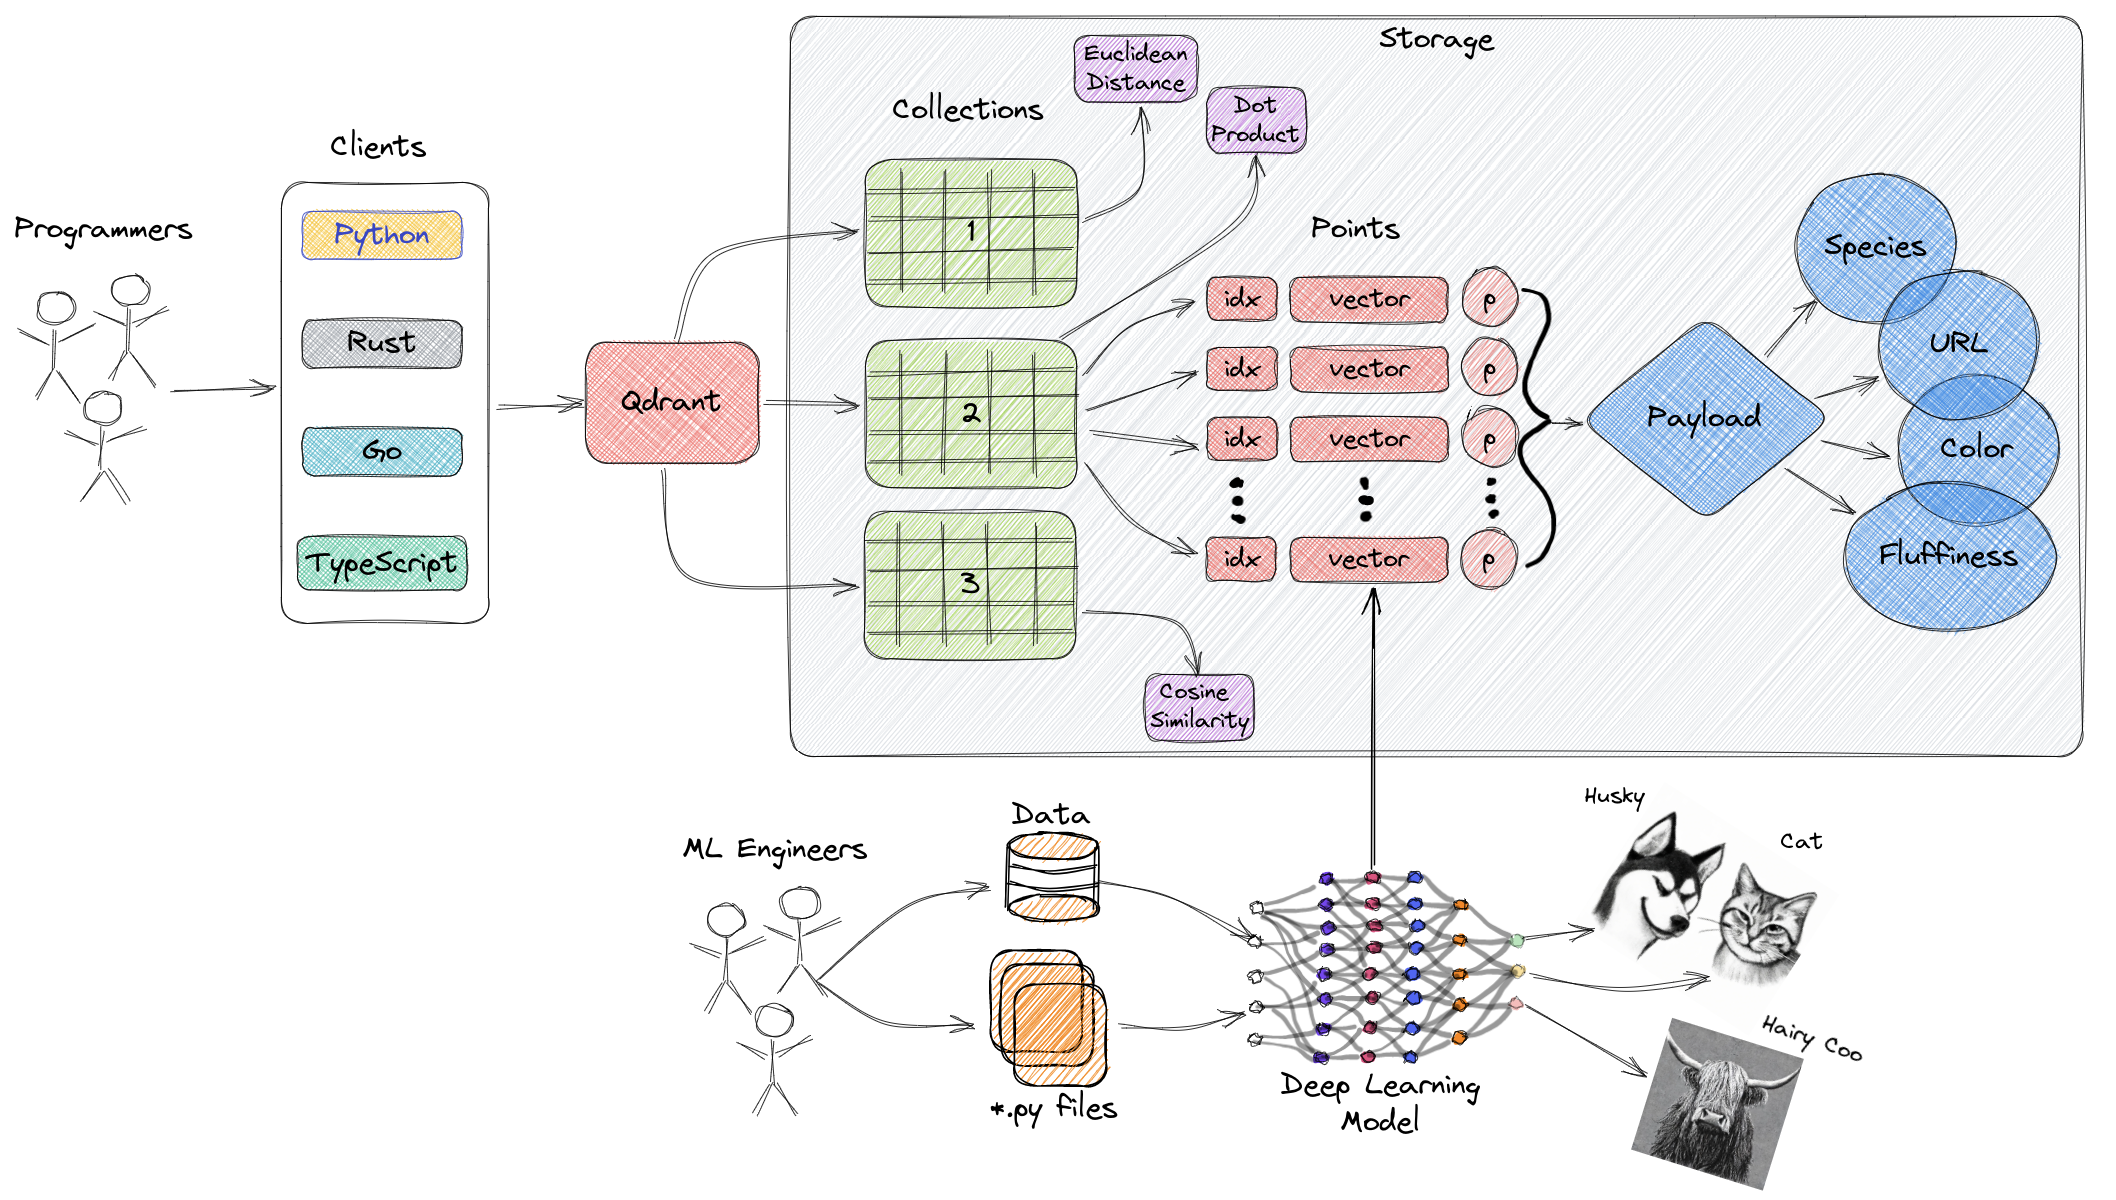
\includegraphics[width=0.7\pdfpagewidth]{images/qdrant_overview.png}
        \caption{Una vista ad alto livello di come è strutturato Qdrant}
    \end{figure}
\end{center}

In conclusione, i database vettoriali sono strumenti essenziali per il trattamento delle informazioni e l'elaborazione del linguaggio naturale. La loro applicazione nei LLM ne potenzia le capacità di comprensione e generazione del testo, contribuendo all'avanzamento delle applicazioni nell'NLP e nei campi connessi.